\subsection{Разработка алгоритма синхронизации данных}
\label{sec:design:sync}

Некоторую функциональность программного обеспечения часто необходимо заложить на стадии проектирования, так как в противном случае реализация таких возможностей может стать слишком накладной или даже невозможной.

Одной из таких функций является возможность синхронизации данных, сохраненных локально, с удаленным сервером для последующей поддержки доступа к приложению с любого устройства.

Данную функциональность не планируется реализовывать в рамках данного проекта, однако необходимо выполнить ее проектирование.

Для успешной реализации алгоритма синхронизации локальной и удалённой баз данных следует упомянуть некоторые особенности проектируемого программного средства:
\begin{itemize}
    \item приложение является однопользовательским;
    \item приложение имеет возможность работы без соединения с сервером;
    \item у пользователя есть возможность управлять практически всеми сущностями в системе, а именно произвольно удалять, изменять и создавать их;
    \item предполагаемый удалённый сервер хранит данные не только одного пользователя;
    \item программное средство не предоставляет возможности просмотра истории изменений той или иной сущности.
\end{itemize}

С учётом этих особенностей, сформулируем список проблем, которые возникают при синхронизации удалённой и локальной баз данных:
\begin{itemize}
    \item дублируемые идентификаторы -- конкретный уникальный идентификатор отдельно взятой сущности может не совпадать в удалённой и локальной версии БД;
    \item определение всех изменений в локальной версии БД -- необходимо знать, какие данные были удалены, изменены и созданы в локальной БД для того, чтобы сообщить об этом удалённому серверу.
\end{itemize}

Для решения проблемы дублируемых идентификаторов необходимо внутри каждой сущности иметь дополнительный, \emph{глобальный} идентификатор, который при создании сущности локально будет заполняться пустым значением.
Впоследствии, после обмена информацией с сервером, данное поле должно заполняться нужным значением.

Проблему определения изменений в локальной БД возможно решить с при помощи ведения \emph{журнала изменений} для каждой сущности.
При каждом действии с сущностью операция должна регистрироваться в данном журнале с занесением всей информации об изменениях в данных, а также типе и времени самой операции.
Синхронизация должна происходить каждый раз при появления возможности интернет-подключения, а также периодически в течении постоянного интернет-соединения.

С учётом описанных выше особенностей, алгоритм синхронизации локальной и удалённой бд должен заключаться в следующем:
\begin{enumerate}
    \item Сервис синхронизации формирует список локальных изменений на основе журналов изменений для каждой сущности.
    При этом во внимание принимается только последнее действие с любым из объектов, так как не требуется хранить сохранять никакой информации об истории изменений объекта.
    \item Удалённый сервер формирует свой список изменений на основе своих журналов.
    \item Список локальных изменений отправляется на удаленный сервер.
    \item Сервер применяет изменения с учётом своего списка, приоритет предоставляется операции над объектом, которая была совершена позже всего.
    Операция удаления также является приоритетной.
    \item Сервер формирует конечный список изменений в данный момент времени и отправляет его клиенту.
    \item Клиент получает конечный список и применяет все переданные изменения для локальной базы данных.
    \item После успешной синхронизации клиент удаляет все изменения в журналах в силу их большей ненадобности.
\end{enumerate}

Схема описанного алгоритма представлена на рисунке~\ref{fig:design:sync:diagram}.

\begin{figure}[p]
    \centering
    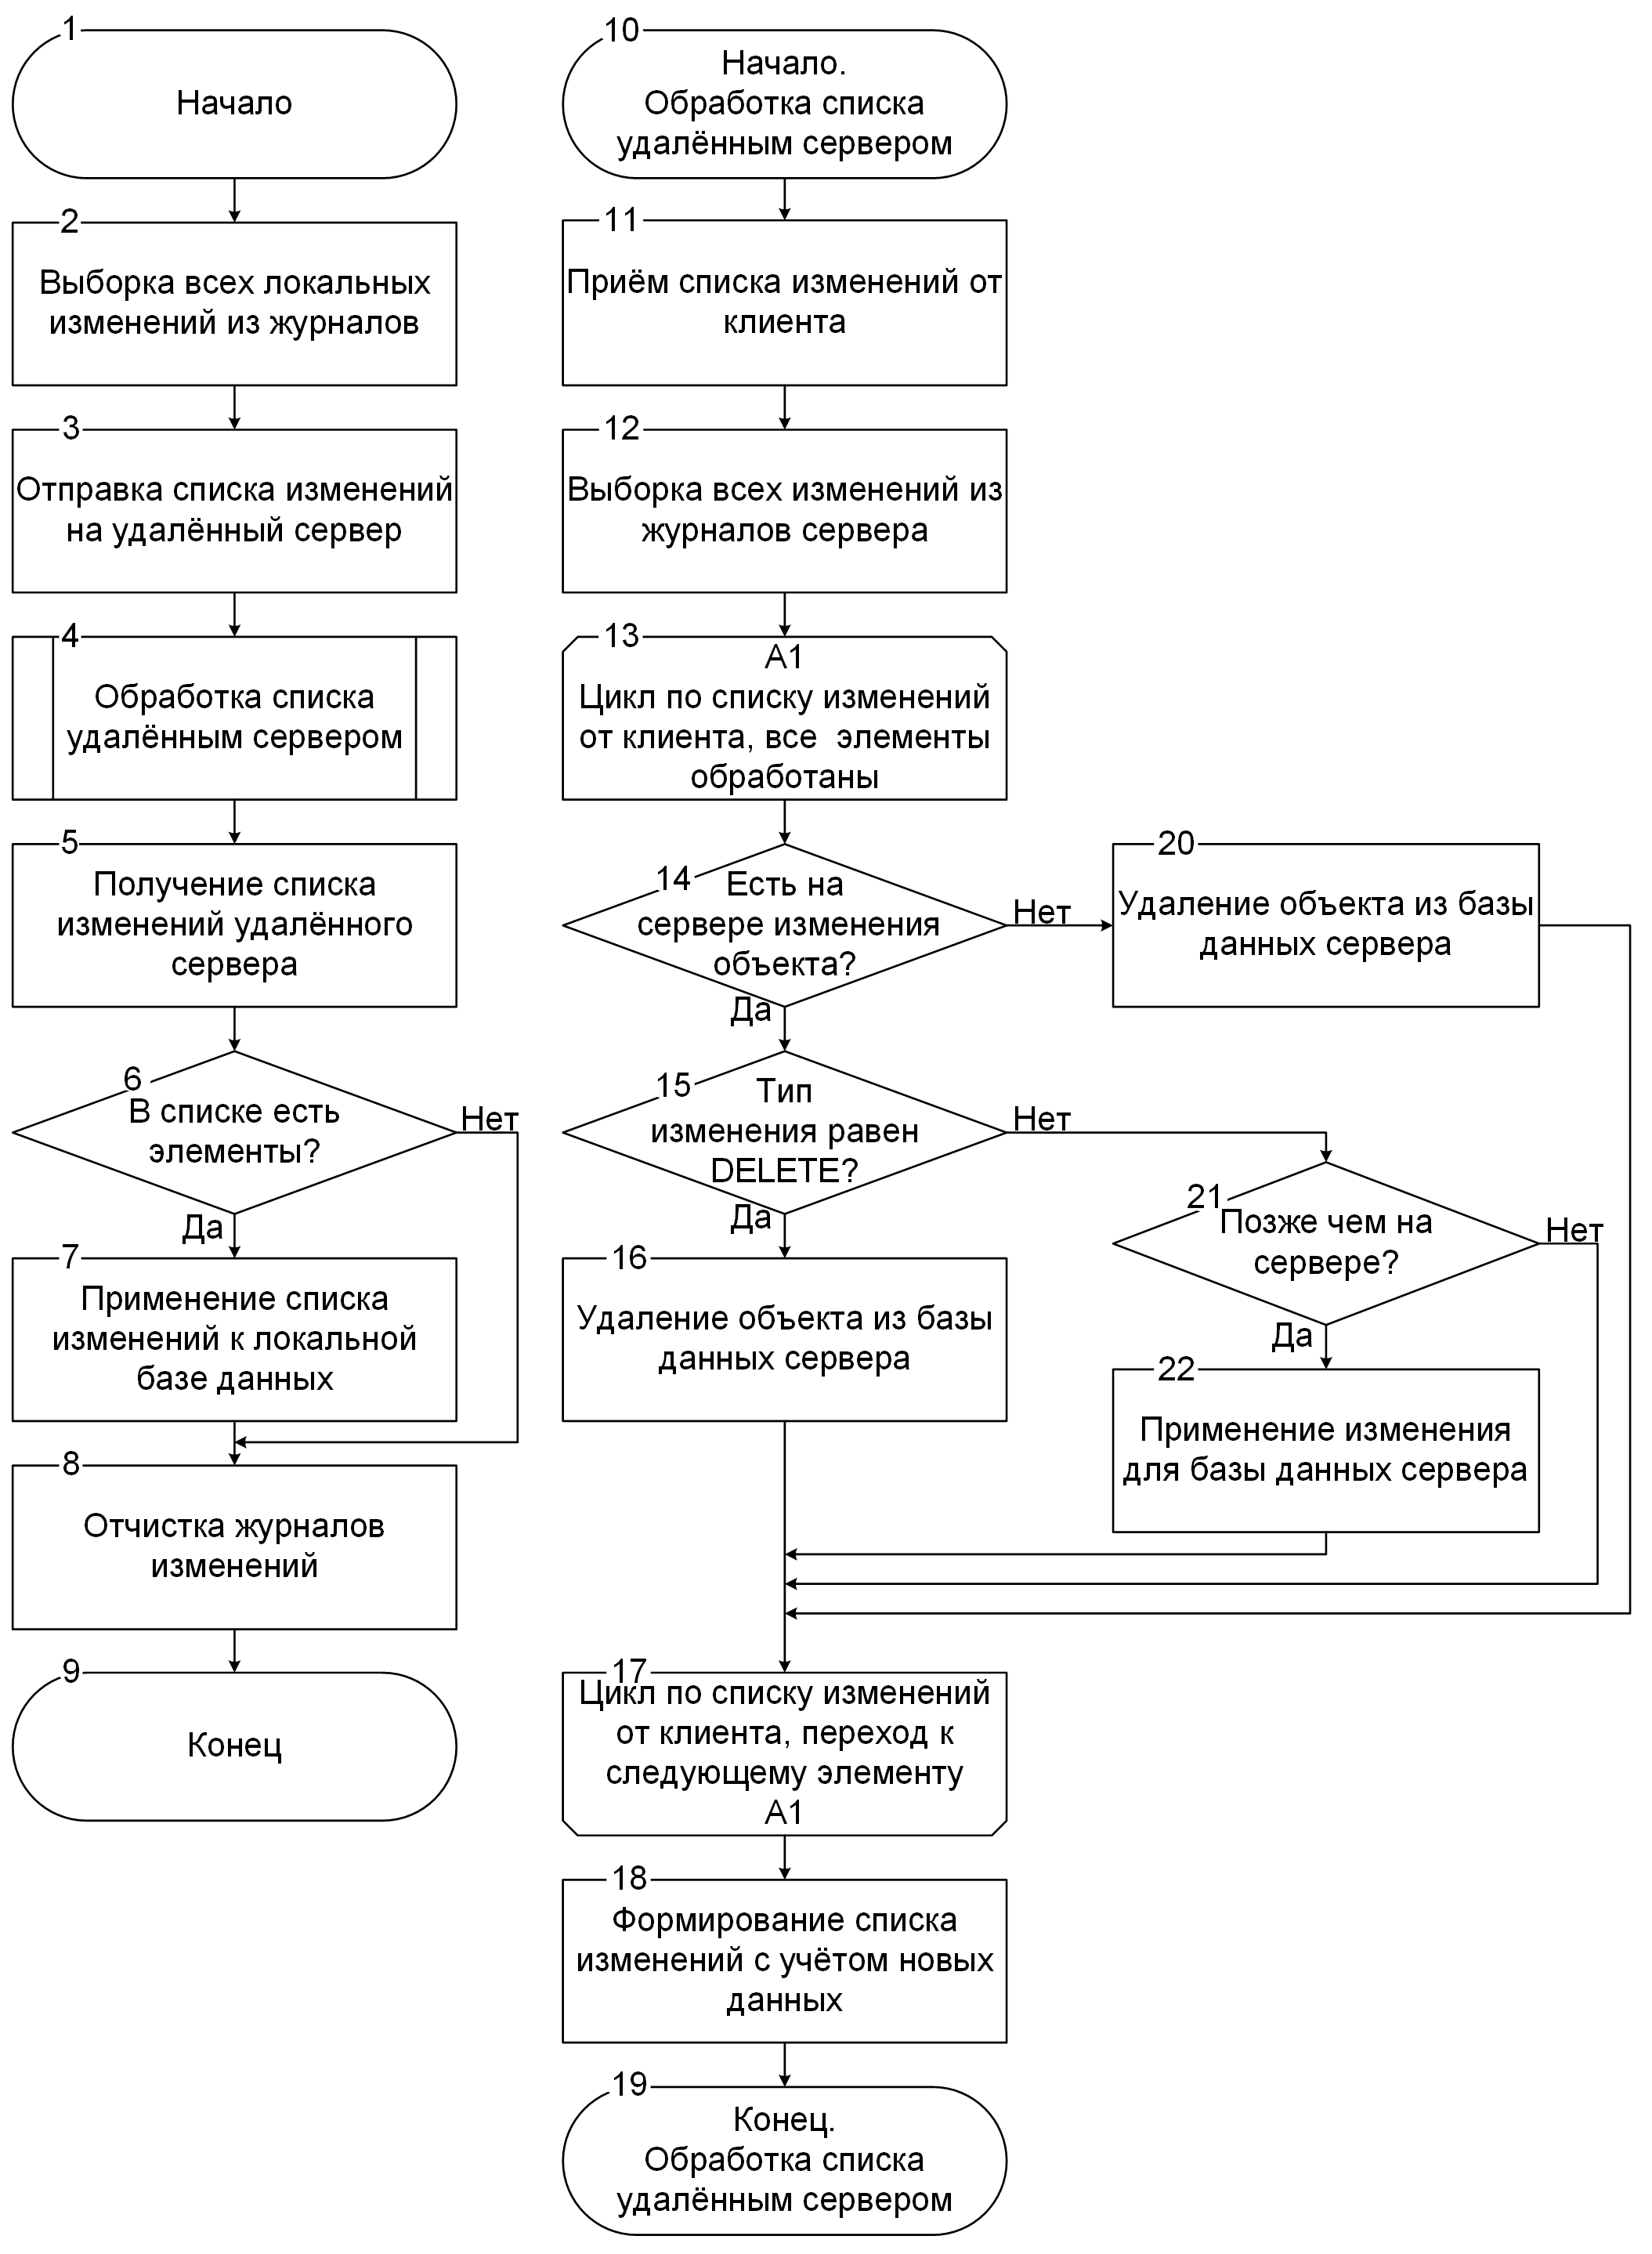
\includegraphics[scale=0.30]{3_2_sync.png}
    \caption{Алгоритм синхронизации локальной и удалённой баз данных}
    \label{fig:design:sync:diagram}
\end{figure}

Описанный алгоритм требует внесения изменений в модель локальной базы данных, которые будут описаны во время разработки базы данных.